\input{"C:/Users/spileggi/Google Drive/STAT 330/Lectures/SlideStyle.tex"}



\title[Lecture 12]{Turning output into data, PROC TRANSPOSE, PROC EXPORT}
\author[Pileggi]{Shannon Pileggi}

\institute[STAT 330]{STAT 330}

\date{}


\begin{document}

\begin{frame}
\titlepage
\end{frame}

\begin{frame}
\frametitle{OUTLINE\qquad\qquad\qquad} \tableofcontents[hideallsubsections]
\end{frame}

%\begin{frame}
%\ft{Motivating problem}
%We'd like to create an external file that contains summary statistics (e.g., mean, standard deviation) of the quantitative variables in the \ttt{acs} data set so that we can include these in a report.
%\vskip20pt
%\oyo Describe a game plan to achieve this.
%\vskip100pt
%\end{frame}


%===========================================================================================================================
\section[Turning output into data]{Turning output into data}
%===========================================================================================================================
\subsection{}
\begin{frame}
\tableofcontents[currentsection, hideallsubsections]
\end{frame}

\begin{frame}
\ft{Overview}
\bi
\item For many procedures you can use an \ttt{OUTPUT} statement or an \ttt{OUT =} option to store printed output to a SAS data set
\item If that option isn't available, you can all use the \ttt{ODS} system to obtain the output
\item This can be helpful for assembling statistics from many pieces of output, either for a succinct table or for a figure
\ei
\end{frame}

\begin{frame}[fragile]
\ft{Data}
\bmp{1.0\textwidth}
\footnotesize
\begin{code}{.0}
PROC IMPORT OUT = WORK.ACS DATAFILE = "&path.acs.csv"
            DBMS = CSV REPLACE;
    GETNAMES = YES;
    DATAROW = 2;
    GUESSINGROWS = 1000 ;
RUN;
\end{code}
\emp
\vskip10pt
\bmp{0.8\textwidth}
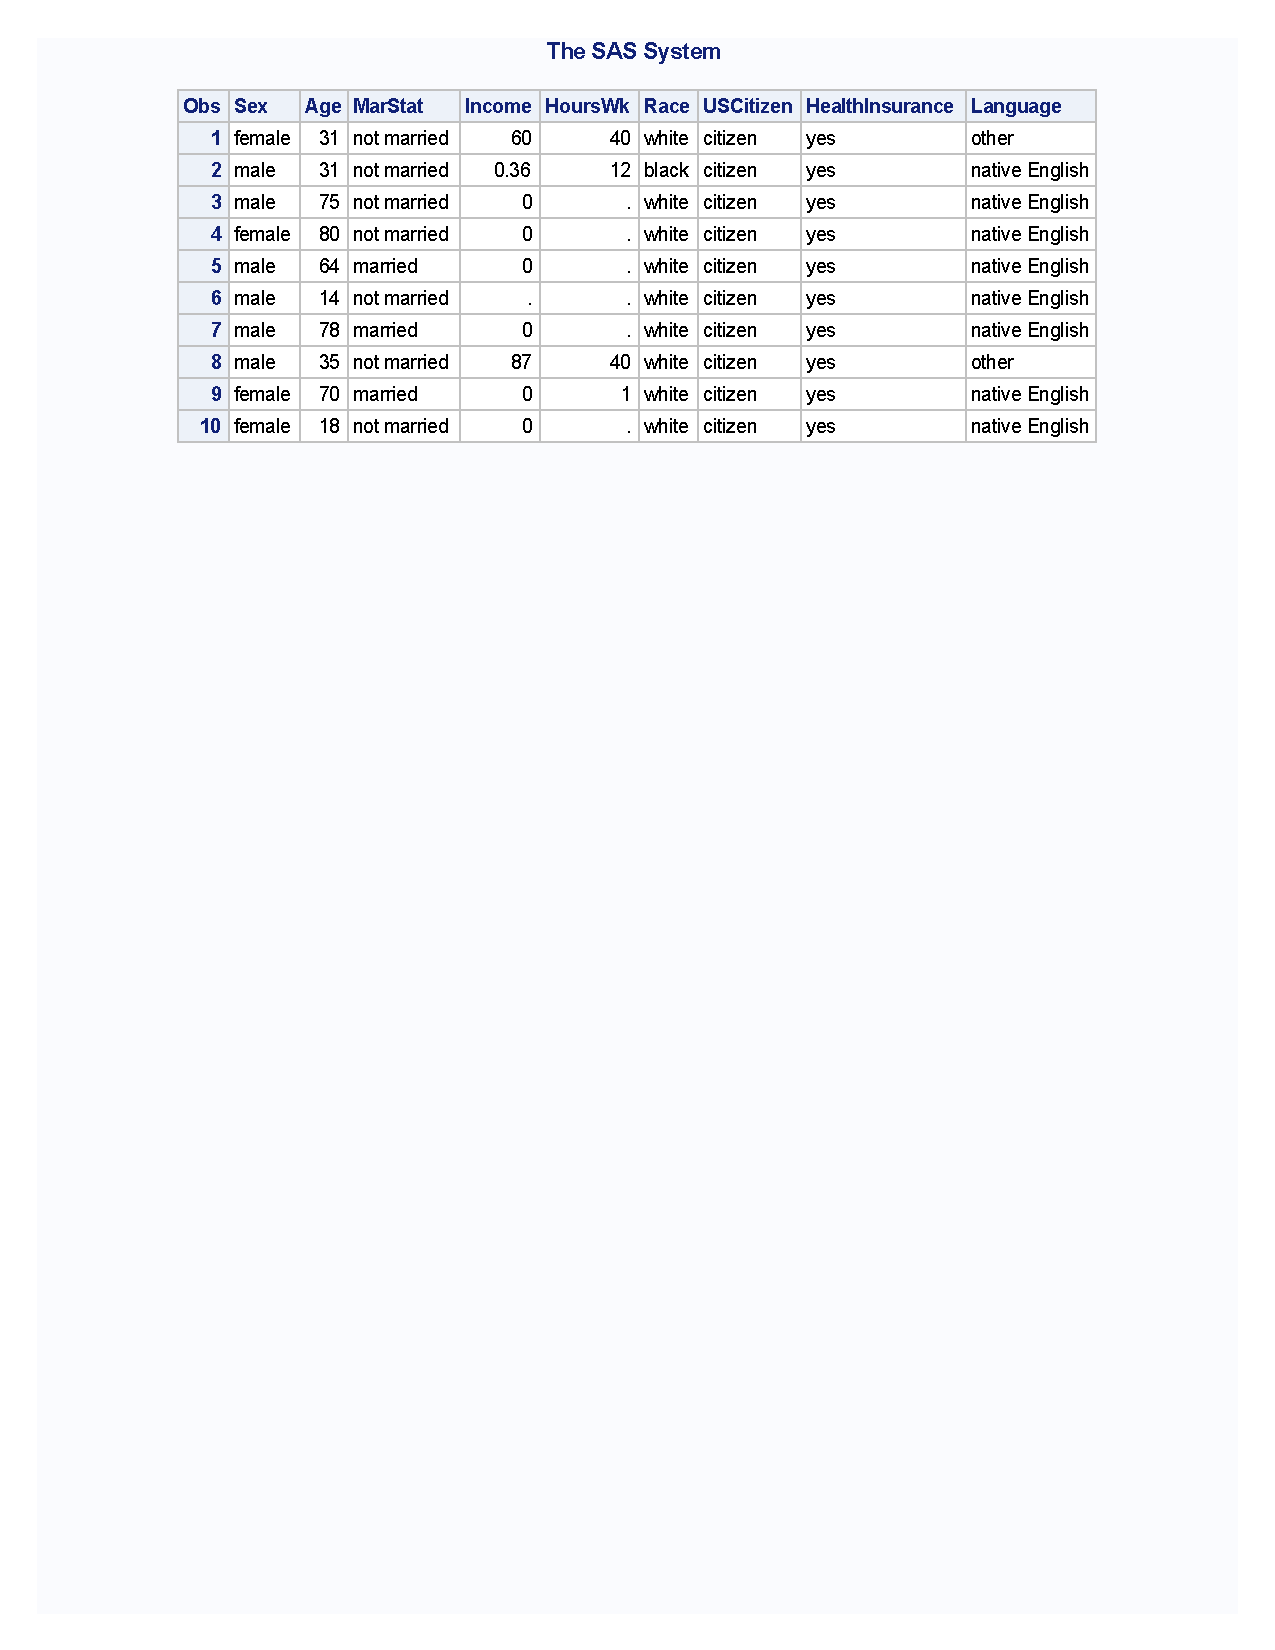
\includegraphics[trim=3cm 18cm 3cm 1.5cm,clip,width=1.0\textwidth]{L12_acs.pdf}
\emp
\end{frame}


\begin{frame}[fragile]
\ft{Storing output from PROC MEANS}
\hspace*{-0.3in}
\bmp{0.55\textwidth}
\footnotesize
\begin{code}{.0}
PROC MEANS DATA = WORK.ACS ;
   \textcolor{OrangeRed}{OUTPUT OUT = meansresults ;}
RUN ;
\end{code}
\vspace{4ex}
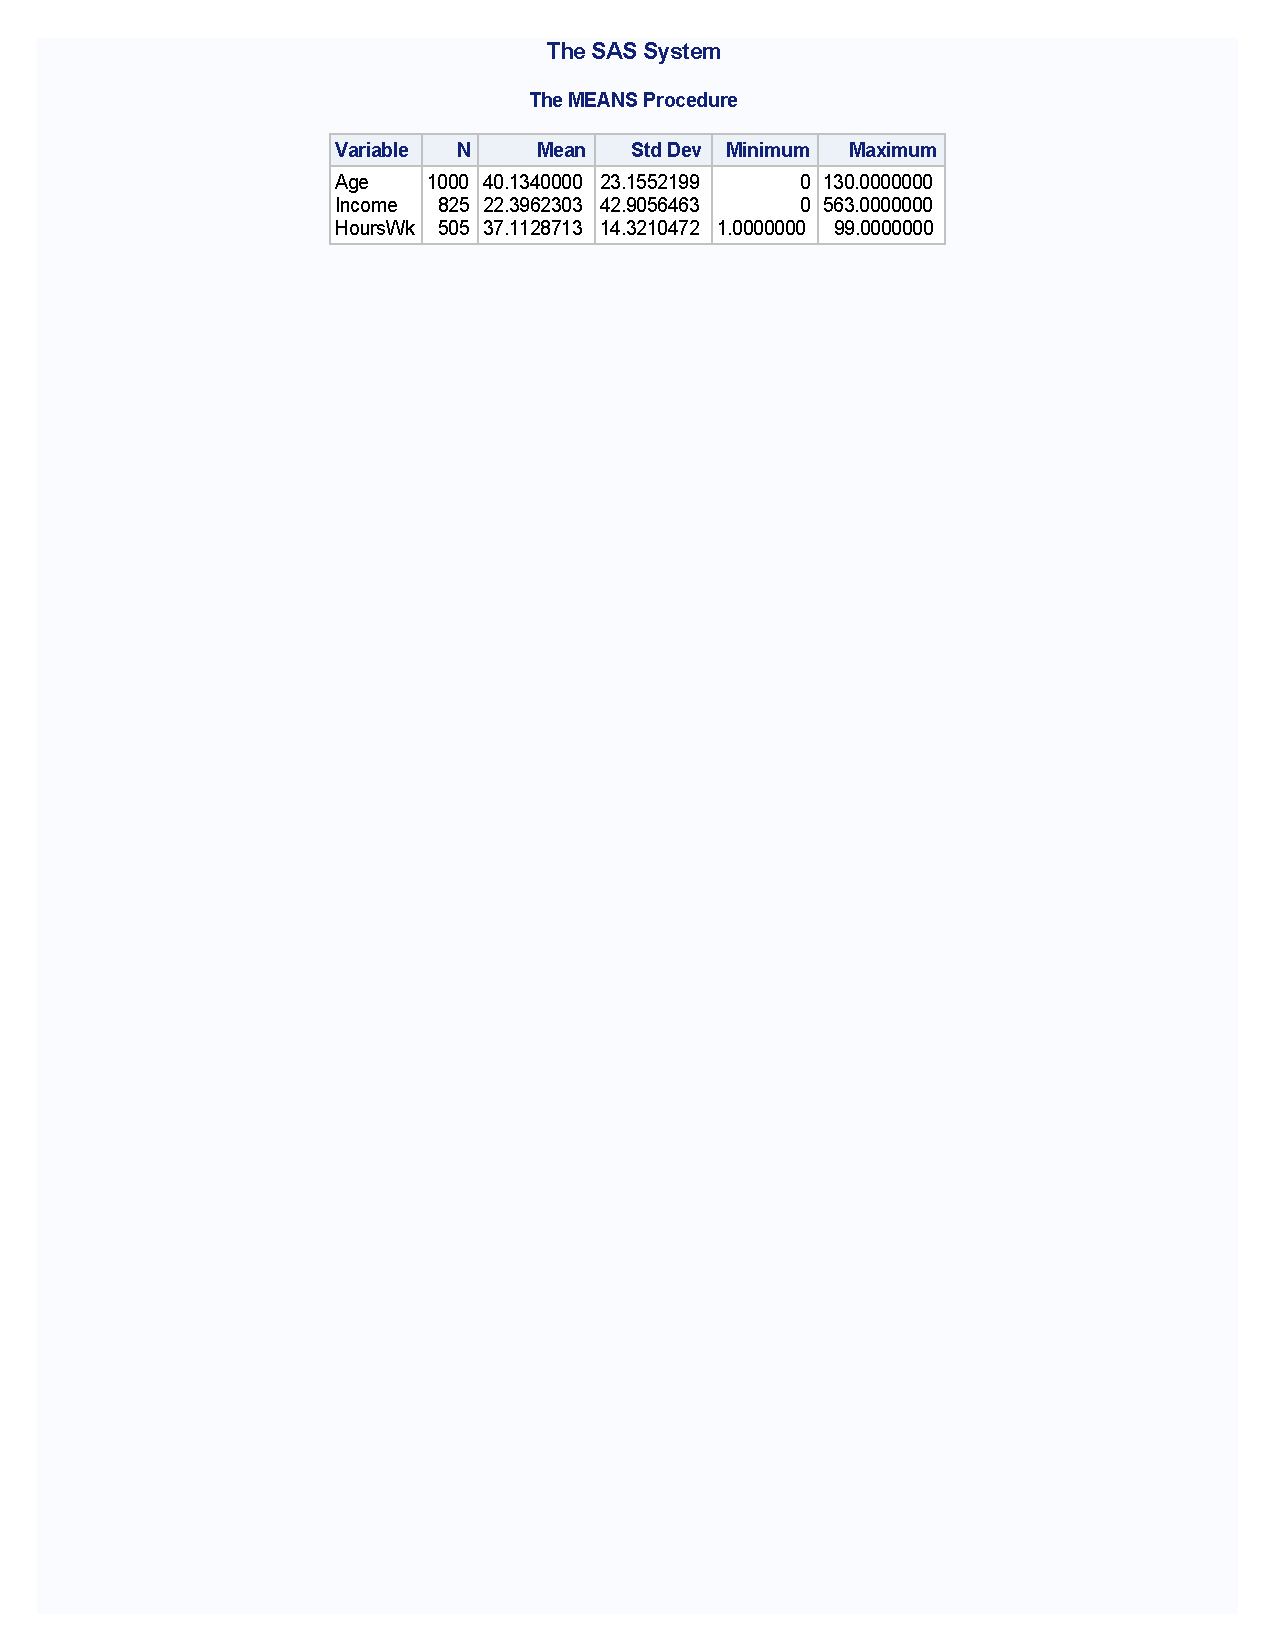
\includegraphics[trim=4cm 18cm 4cm 2.0cm,clip,width=1.0\textwidth]{L12_pmeans.pdf}
\emp
\bmp{0.03\textwidth} \hspace{0.5in} \emp
\bmp{0.55\textwidth}
\footnotesize
\begin{code}{.0}
PROC PRINT DATA = \textcolor{OrangeRed}{meansresults} ;
RUN ;

\end{code}
\vspace{2ex}
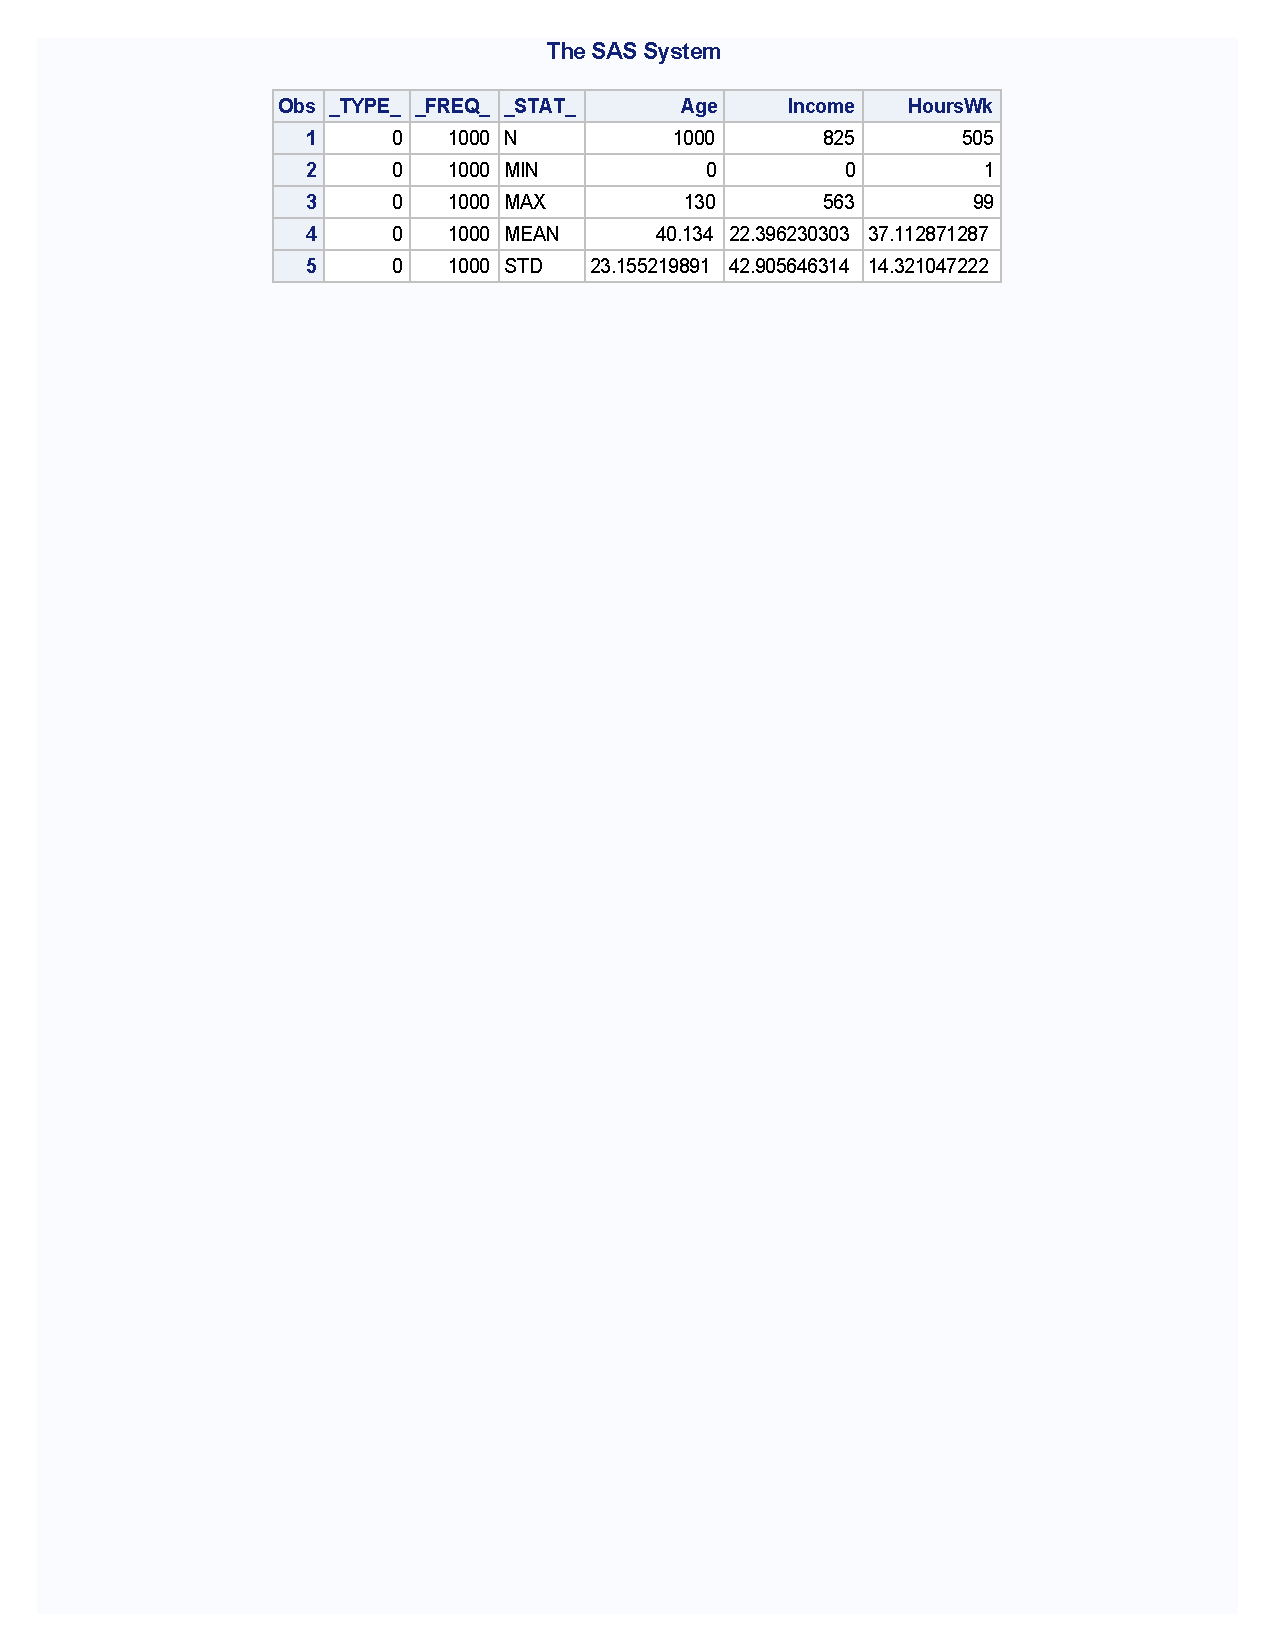
\includegraphics[trim=4cm 18cm 4cm 1.5cm,clip,width=1.0\textwidth]{L12_pmeansout.pdf}
\emp
\end{frame}

\begin{frame}[fragile]
\ft{Storing output from PROC FREQ}
\hspace*{-0.3in}
\bmp{0.55\textwidth}
\footnotesize
\begin{code}{.0}
PROC FREQ DATA = WORK.acs ;
   TABLES sex*marstat /
       \textcolor{OrangeRed}{OUT = freqresults} ;
RUN ;
\end{code}
\vspace{2ex}
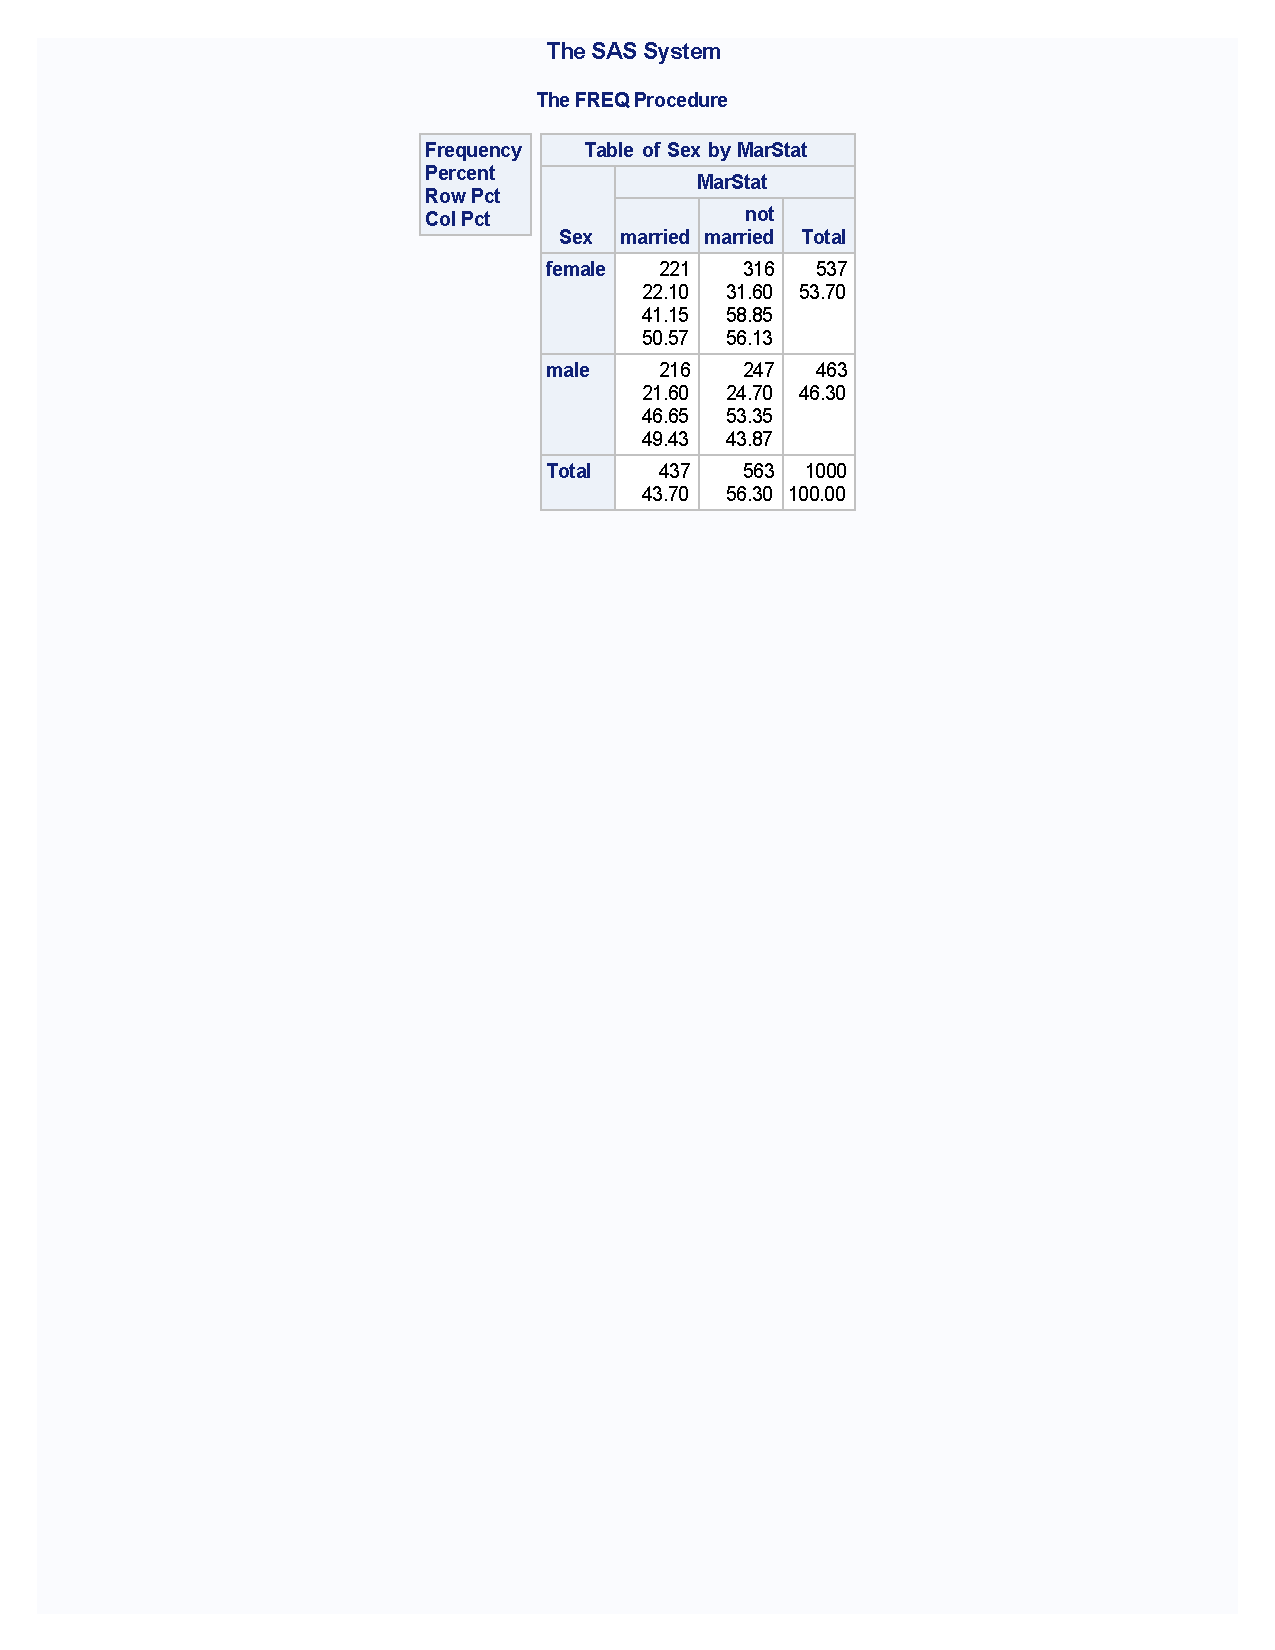
\includegraphics[trim=5cm 19cm 5cm 2.0cm,clip,width=1.0\textwidth]{L12_pfreq.pdf}
\emp
\bmp{0.03\textwidth} \hspace{0.5in} \emp
\bmp{0.55\textwidth}
\footnotesize
\begin{code}{.0}
PROC PRINT DATA = \textcolor{OrangeRed}{freqresults} ;
RUN ;


\end{code}
\vspace{2ex}
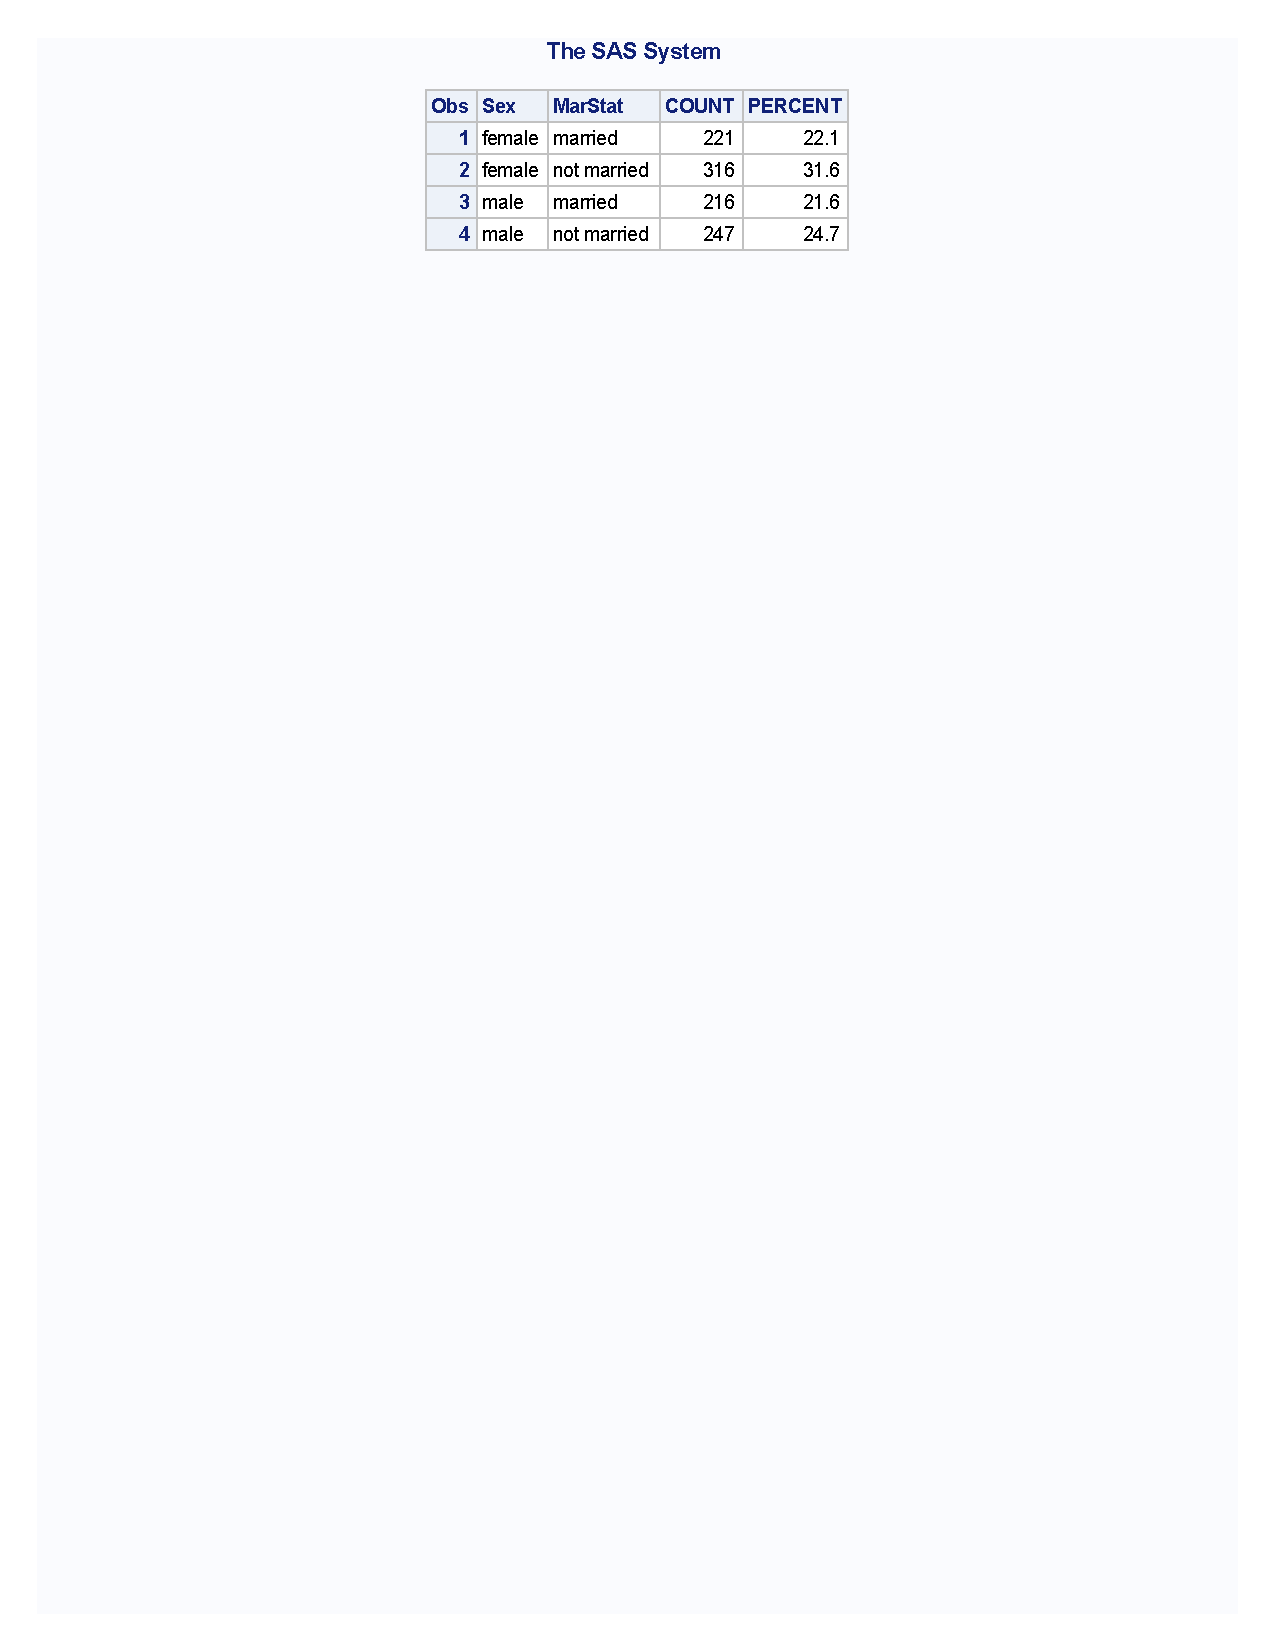
\includegraphics[trim=5cm 19cm 5cm 1.5cm,clip,width=1.0\textwidth]{L12_pfreqout.pdf}
\emp
%Note: you can use an \ttt{OUTPUT} statement in \ttt{PROC FREQ}, but this is used more for inferential rather than descriptive statistics.
\end{frame}

\begin{frame}
\ft{Storing output from PROC TTEST}
PROC TTEST does not have an \ttt{OUTPUT} statement or an \ttt{OUT = } option!  To store results, we need to use ODS.
\begin{enumerate}
\item \emph{Trace} your results from a SAS procedure.
\item Identify the output that you want from your log window.
\item Modify your SAS procedure code to use ODS to store your results.
\end{enumerate}
\end{frame}

\begin{frame}[fragile]
\ft{Step 1 - trace your results}
\hspace*{-0.3in}
\bmp{0.6\textwidth}
\footnotesize
\begin{code}{.0}
\textcolor{OrangeRed}{ODS TRACE ON ;}
PROC TTEST DATA = WORK.acs H0 = 40 ;
   VAR HoursWk ;
RUN ;
\textcolor{OrangeRed}{ODS TRACE OFF ;}
\end{code}
\emp
\bmp{0.03\textwidth} \hspace{1in} \emp
\bmp{0.5\textwidth}
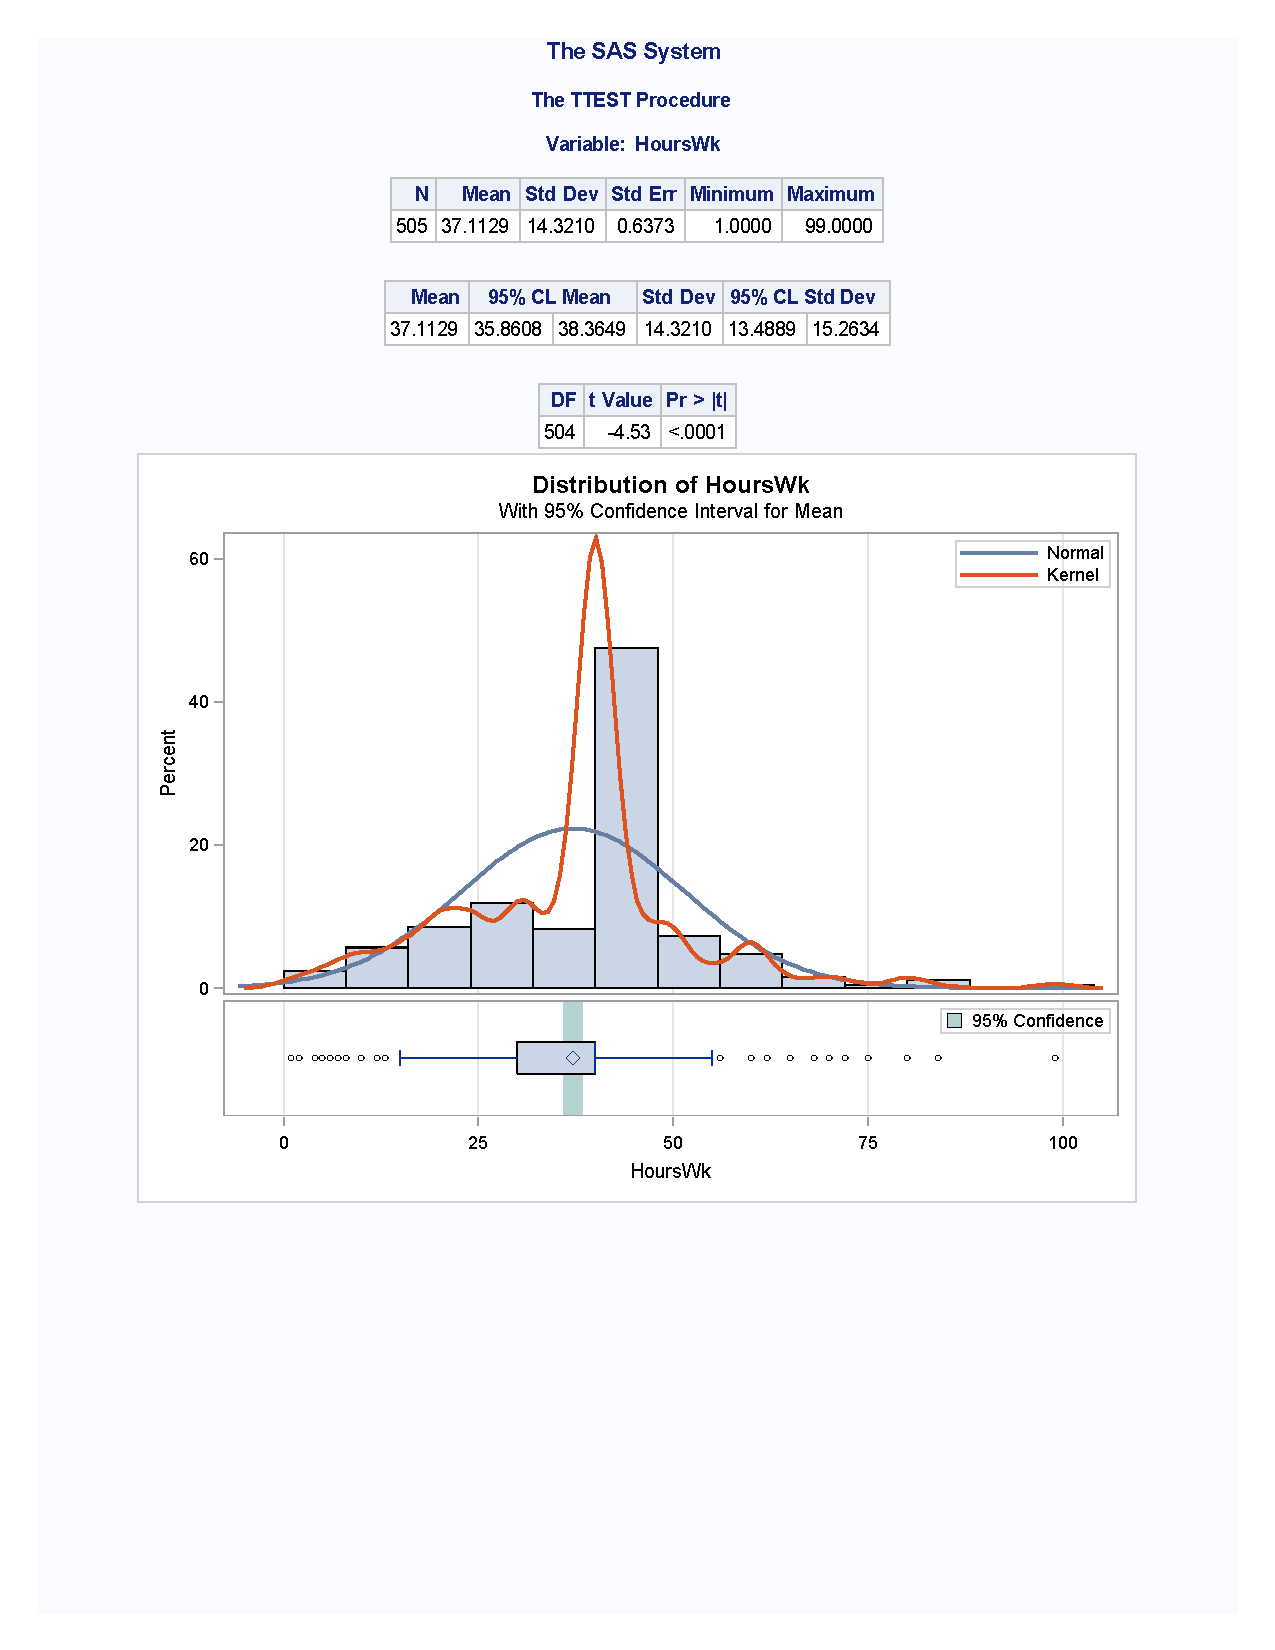
\includegraphics[trim=6.5cm 20.3cm 6.5cm 1.5cm,clip,width=0.8\textwidth]{L12_pttest.pdf}
\emp
\end{frame}

\begin{frame}[fragile]
\ft{Step 2 - examine log}
There are five pieces of output that I can grab! (4 shown)
\hspace*{-0.3in}
\bmp{0.60\textwidth}
\begin{tinycraw}{.0}{From SAS log}
Output Added:
-------------
Name:       Statistics
Label:      Statistics
Template:   Stat.TTest.Statistics
Path:       Ttest.HoursWk.Statistics
-------------

Output Added:
-------------
Name:       \textcolor{OrangeRed}{ConfLimits}
Label:      Confidence Limits
Template:   Stat.TTest.ConfLimits
Path:       Ttest.HoursWk.ConfLimits
-------------
\end{tinycraw}
\emp
\bmp{0.03\textwidth} \hspace{1in} \emp
\bmp{0.55\textwidth}
\footnotesize
\begin{tinycraw}{.0}{From SAS log}
Output Added:
-------------
Name:       TTests
Label:      T-Tests
Template:   Stat.TTest.TTests
Path:       Ttest.HoursWk.TTests
-------------

Output Added:
-------------
Name:       SummaryPanel
Label:      Summary Panel
Template:   Stat.TTest.Graphics.Summary1
Path:       Ttest.HoursWk.SummaryPanel
-------------
\end{tinycraw}
\emp
\end{frame}


\begin{frame}[fragile]
\ft{Step 3 - use ODS to store results}
\hspace*{-0.3in}
\bmp{0.62\textwidth}
\footnotesize
\begin{code}{.0}
PROC TTEST DATA = WORK.acs H0 = 40 ;
  VAR HoursWk ;
  ODS OUTPUT ConfLimits = \textcolor{OrangeRed}{CIresults} ;
RUN ;
\end{code}
\vspace{2ex}
\begin{center}
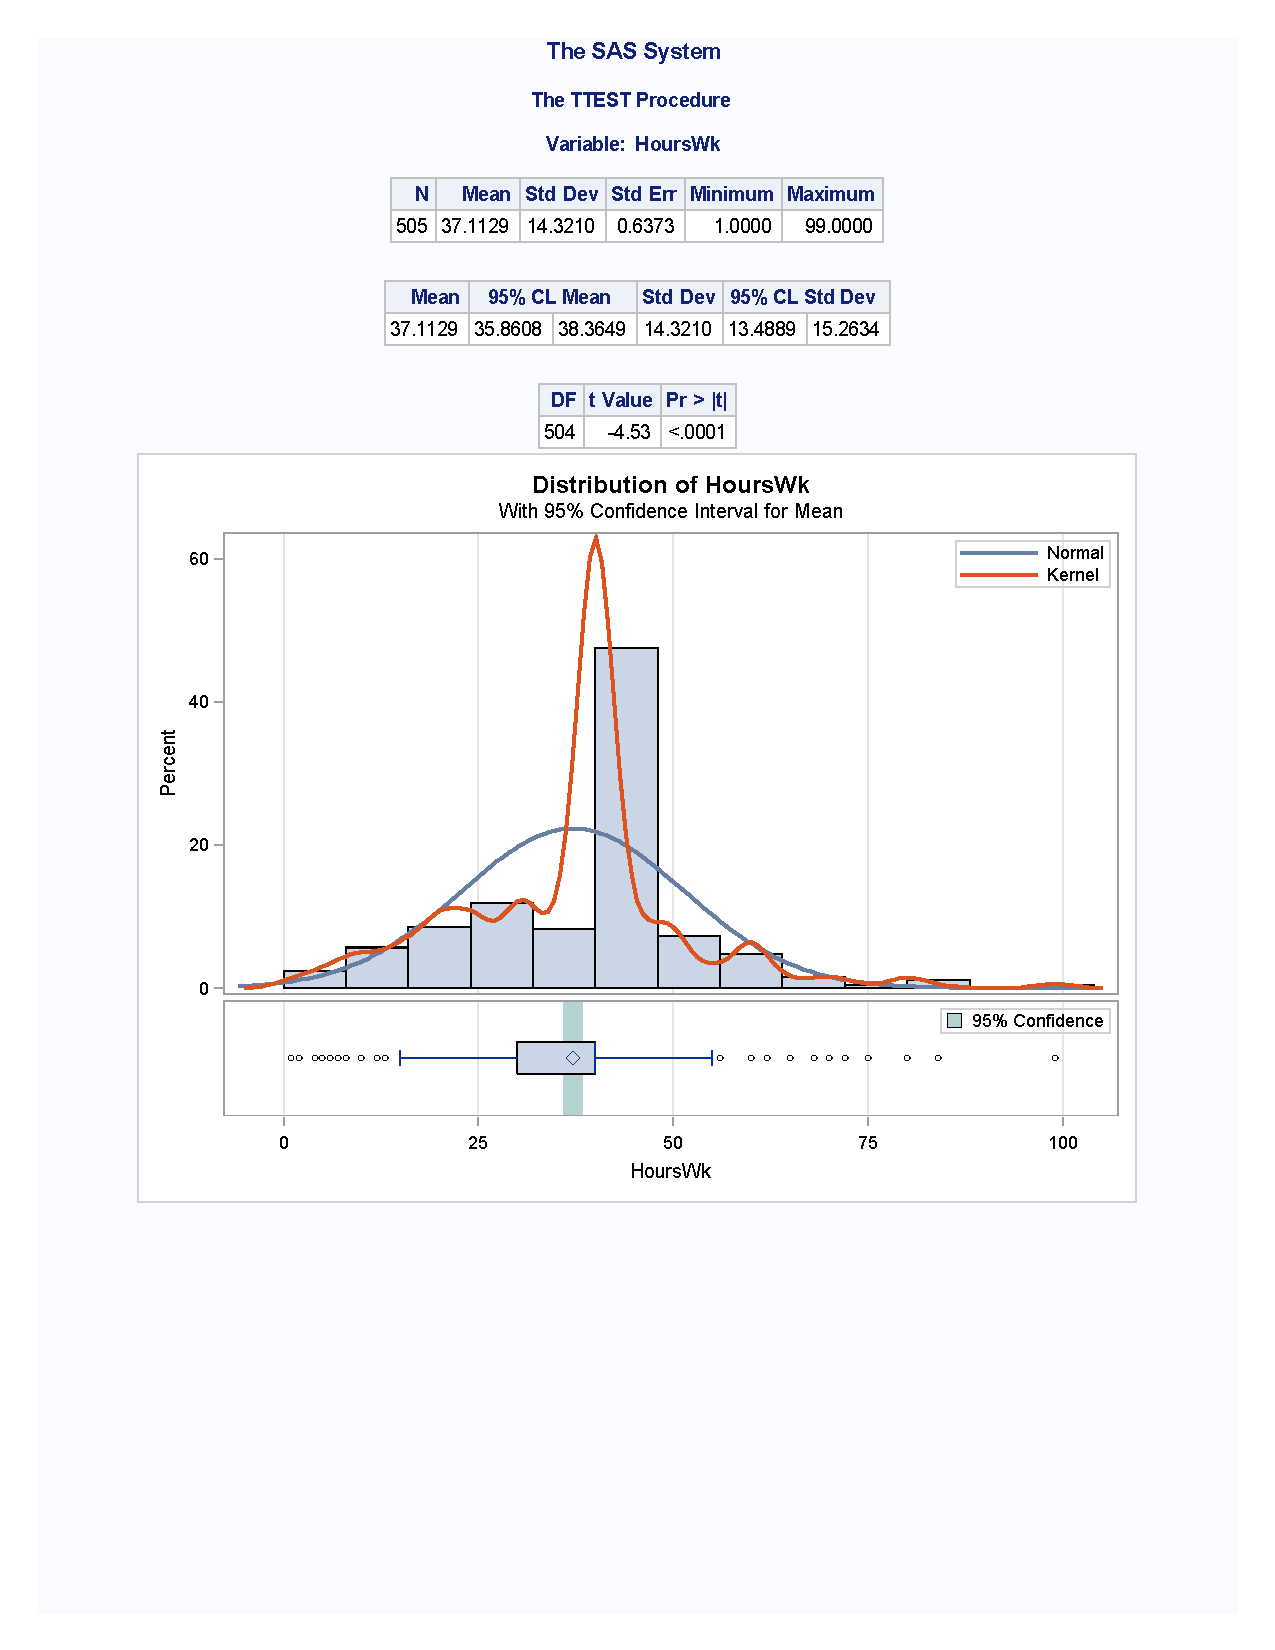
\includegraphics[trim=6.5cm 20.3cm 6.5cm 1.5cm,clip,width=0.7\textwidth]{L12_pttest.pdf}
\end{center}
\emp
\bmp{0.03\textwidth} \hspace{0.5in} \emp
\bmp{0.48\textwidth}
\footnotesize
\begin{code}{.0}
PROC PRINT DATA = \textcolor{OrangeRed}{CIresults};
RUN ;


\end{code}
\vspace{2ex}
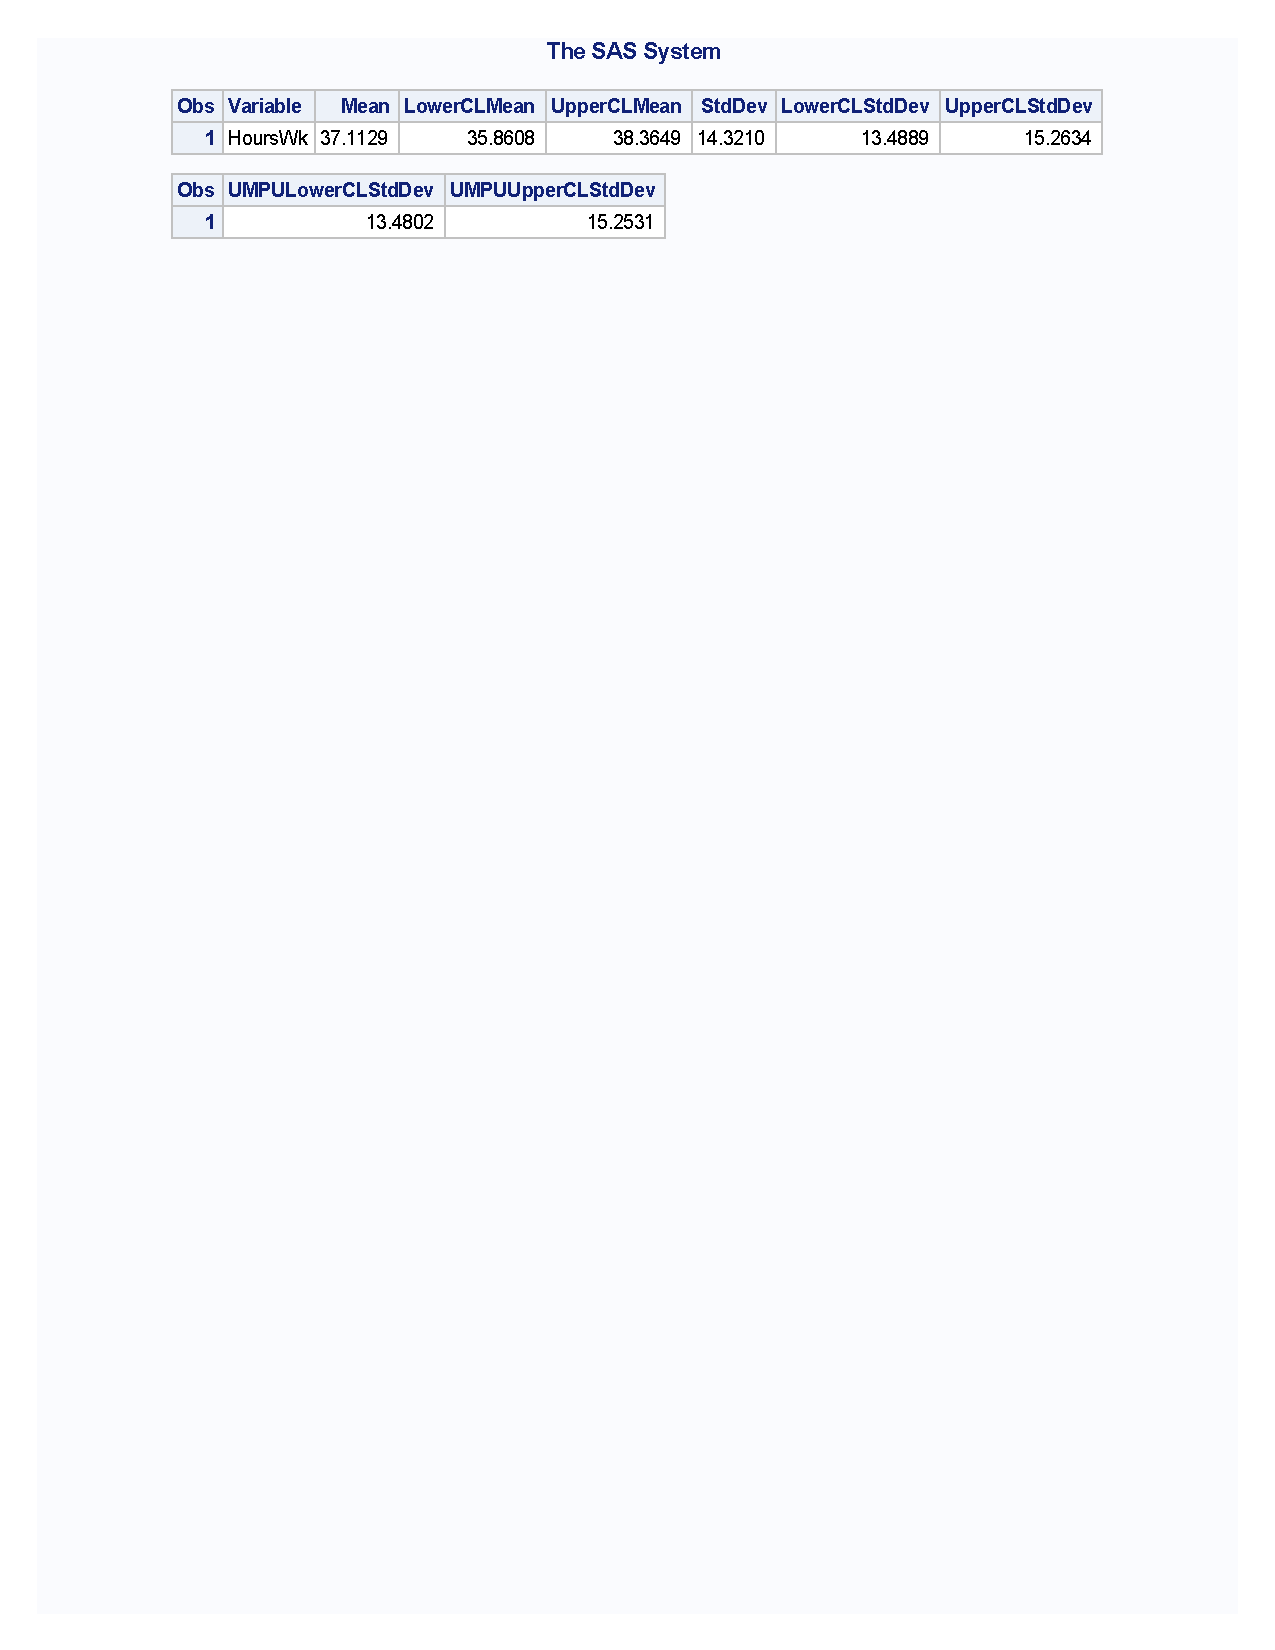
\includegraphics[trim=2cm 17cm 2cm 1.5cm,clip,width=1.0\textwidth]{L12_pttestout.pdf}
\vspace{5ex}
\emp
\end{frame}

%===========================================================================================================================
\section[PROC TRANSPOSE]{PROC TRANSPOSE}
%===========================================================================================================================
\subsection{}
\begin{frame}
\tableofcontents[currentsection, hideallsubsections]
\end{frame}

\begin{frame}[fragile]
\ft{Storing output from PROC MEANS}
\hspace*{-0.3in}
\bmp{0.55\textwidth}
\footnotesize
\begin{code}{.0}
PROC MEANS DATA = WORK.ACS ;
   \textcolor{OrangeRed}{OUTPUT OUT = meansresults ;}
RUN ;
\end{code}
\vspace{4ex}
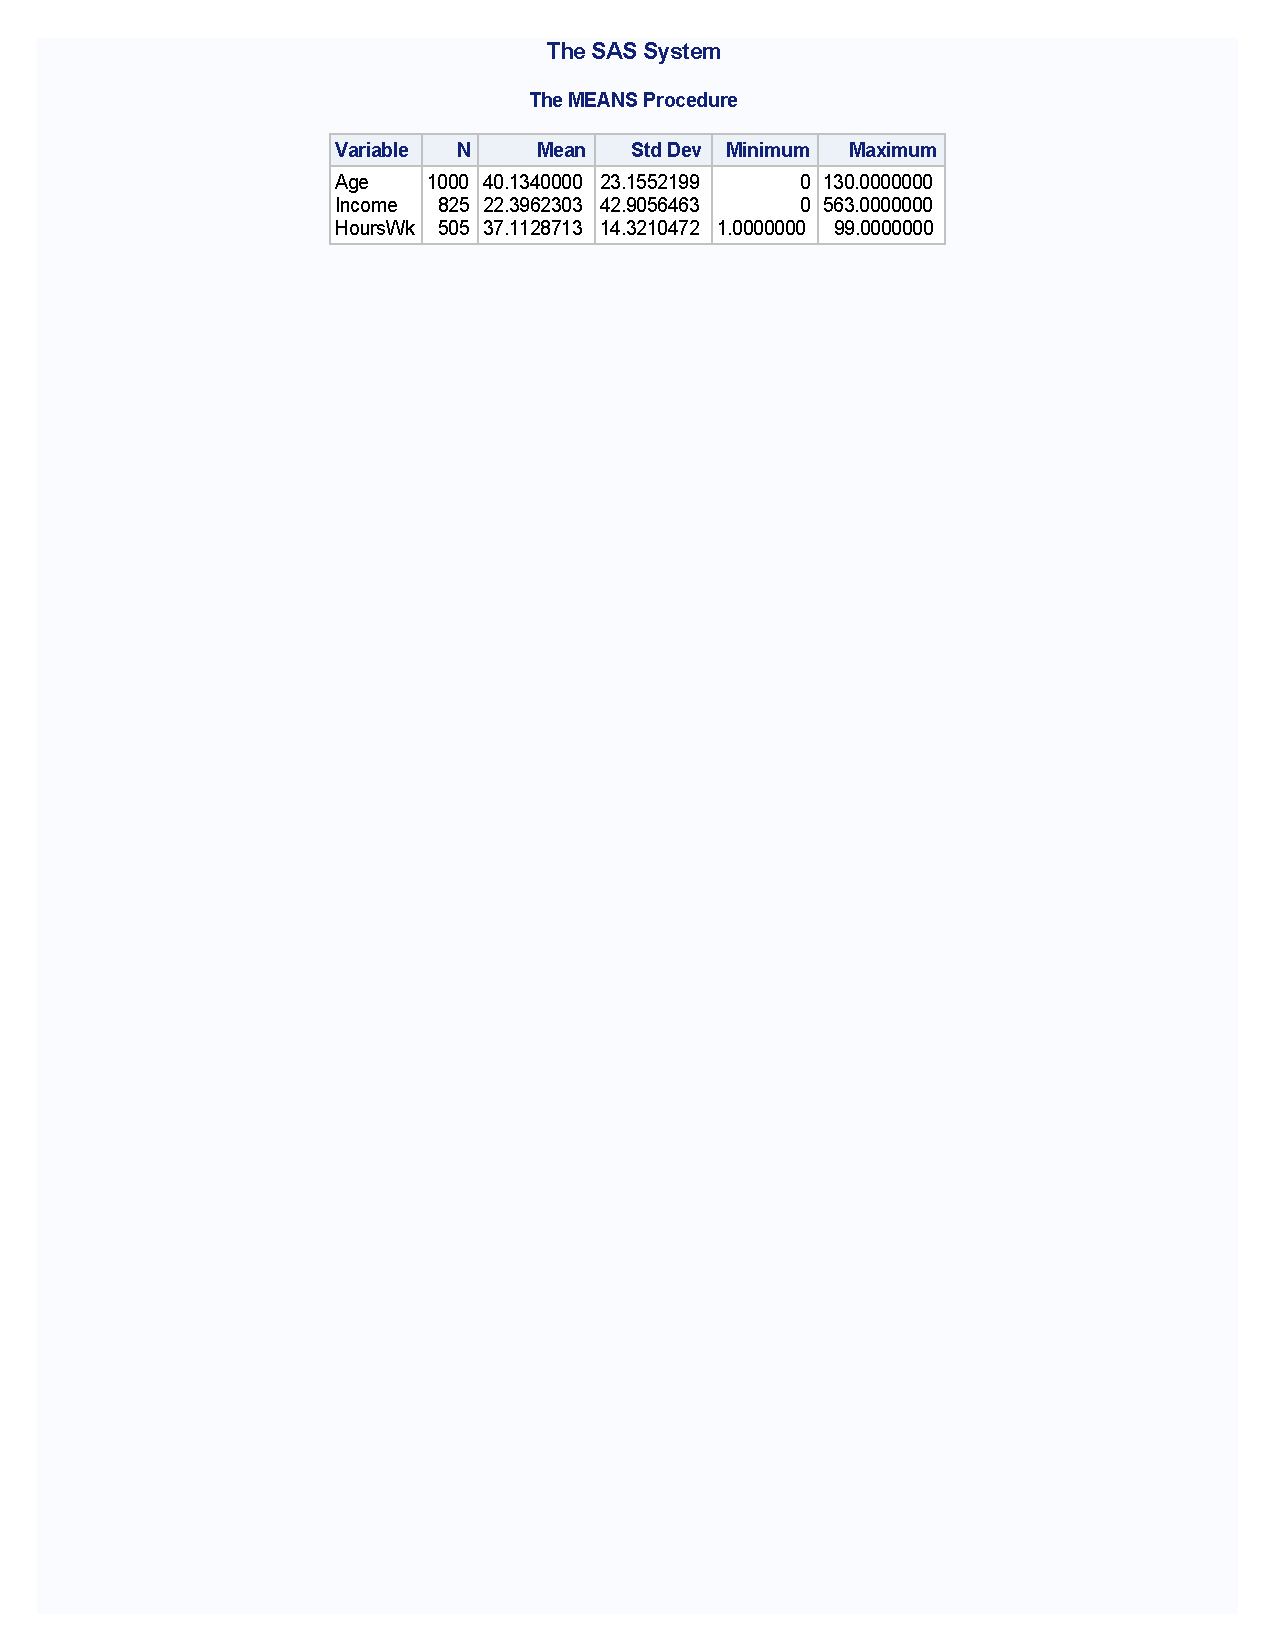
\includegraphics[trim=4cm 18cm 4cm 2.0cm,clip,width=1.0\textwidth]{L12_pmeans.pdf}
\emp
\bmp{0.03\textwidth} \hspace{0.5in} \emp
\bmp{0.55\textwidth}
\footnotesize
\begin{code}{.0}
PROC PRINT DATA = \textcolor{OrangeRed}{meansresults} ;
RUN ;

\end{code}
\vspace{2ex}
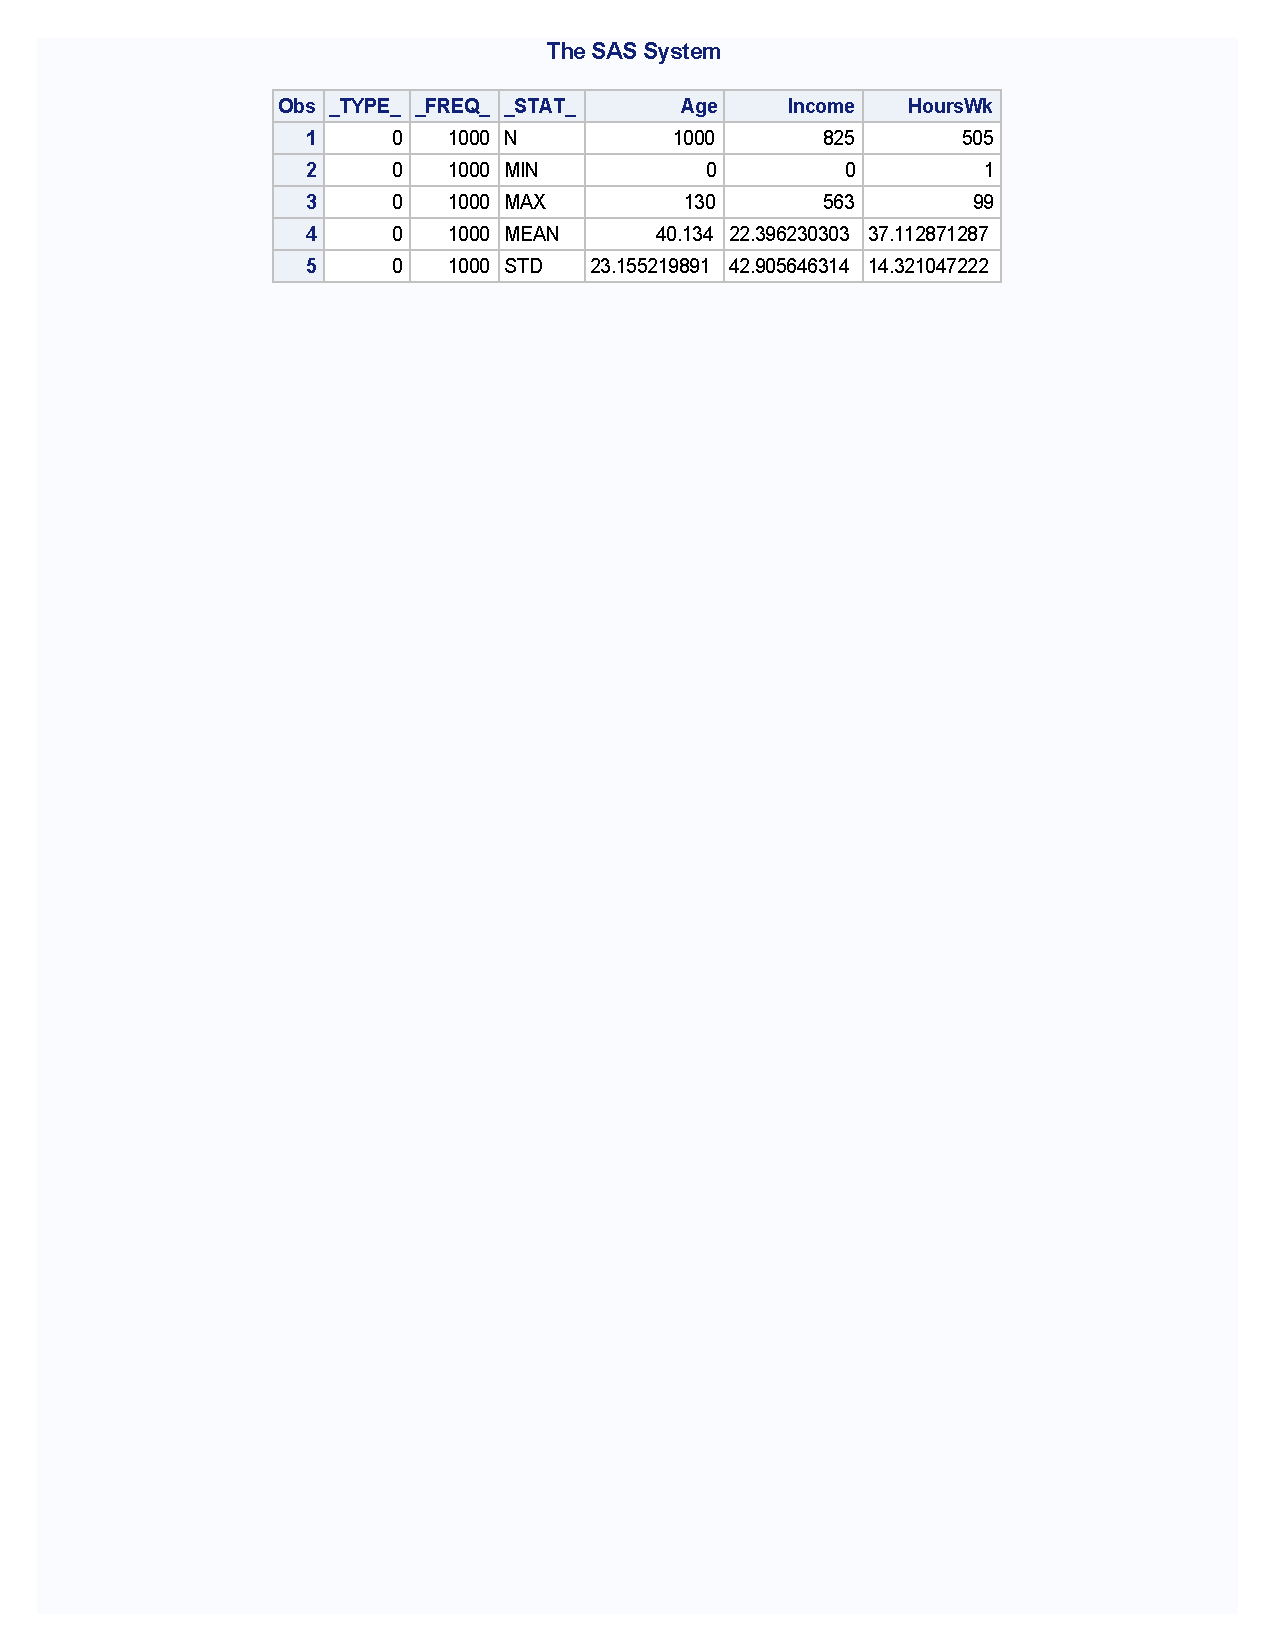
\includegraphics[trim=4cm 18cm 4cm 1.5cm,clip,width=1.0\textwidth]{L12_pmeansout.pdf}
\emp\\
\oyo How can we get our \textcolor{OrangeRed}{meansresults} to look like the original output?
\end{frame}



\begin{frame}[fragile]
\ft{PROC TRANSPOSE}
\hspace*{-0.3in}
\bmp{1.1\textwidth}
\footnotesize
\begin{code}{.0}
PROC TRANSPOSE
   DATA = \emph{DataSetName} OUT = \emph{TransposedData} NAME = \emph{NewVariableName};
   ID \emph{IdentifyingVariable} ;
   BY \emph{GroupingVariable} ;
   VAR \emph{var1} \emph{var2} \emph{var3} ;
RUN;
\end{code}
\emp
\vskip5pt
\bi
\bmp{0.35\textwidth}
\item[\fbox{\ttt{DATA=}}] specifies the SAS data set name you want to transpose
\item[\fbox{\ttt{OUT=}}] name of new transposed data set
\item[\fbox{\ttt{NAME=}}] names a variable in \emph{TransposedData} that contains \ttt{VAR} variables
\emp
\bmp{0.15\textwidth} \hspace{0.05in} \emp
\bmp{0.45\textwidth}
\item[\fbox{\ttt{ID}}] a variable in \emph{DataSetName} that names multiple variables in \emph{TransposedData}
\item[\fbox{\ttt{BY}}] transposes by groups (data must be pre-sorted)
\item[\fbox{\ttt{VAR}}] lists variables to transpose
\item[]
\item[]
\emp
\ei
\end{frame}




\begin{frame}[fragile]
\ft{Transpose summary statistics}
%\bmp{0.08\textwidth} \hspace{0.05in} \emp
\hspace*{-0.3in}
\bmp{0.75\textwidth}
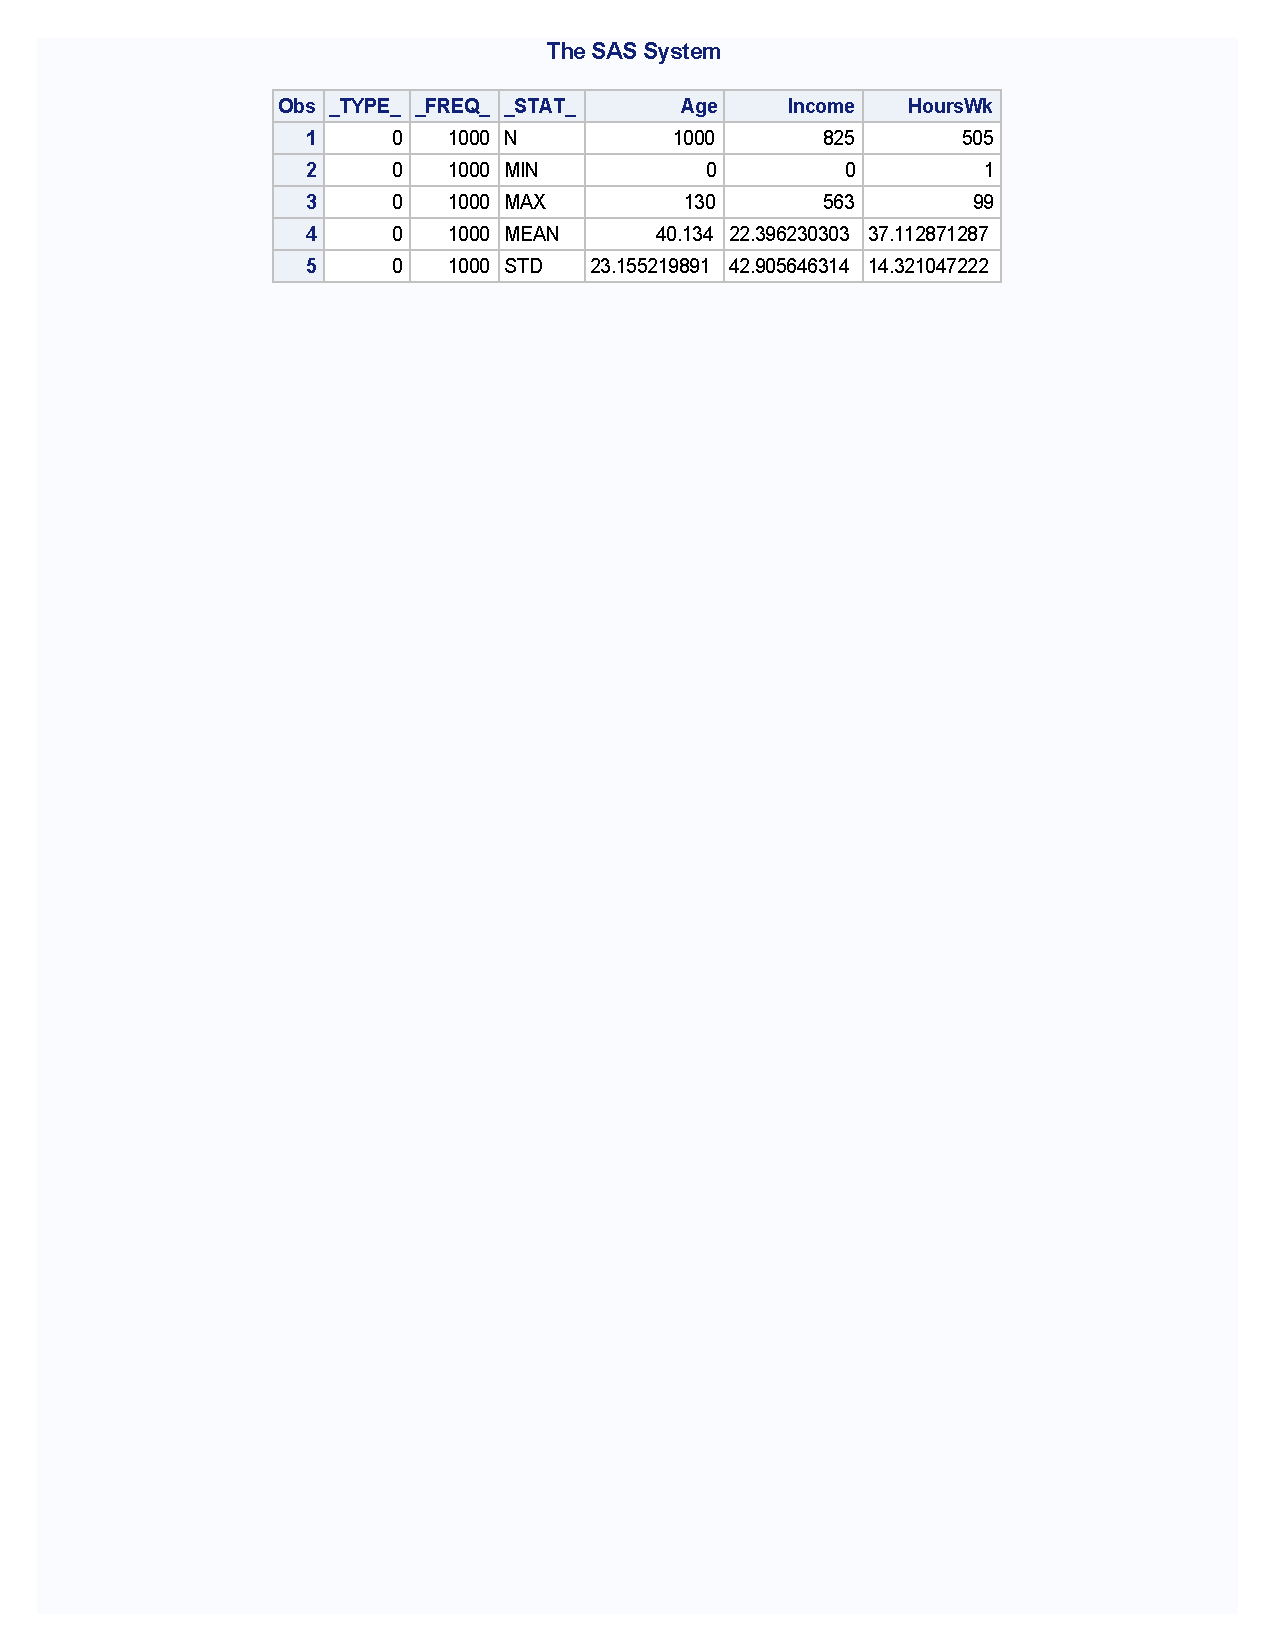
\includegraphics[trim=4cm 22cm 4cm 0.5cm,clip,width=1.0\textwidth]{L12_pmeansout.pdf}
\emp
\vskip5pt
\hspace*{-0.3in}
\bmp{0.45\textwidth}
\footnotesize
\begin{code}{.0}
PROC TRANSPOSE
   DATA = meansresults
   OUT = statstransposed
   NAME = variable ;
   ID _stat_ ;
   VAR age income hourswk;
RUN ;
\end{code}
\emp
\bmp{0.03\textwidth} \hspace{0.05in} \emp
\bmp{0.66\textwidth}
\vspace{5ex}
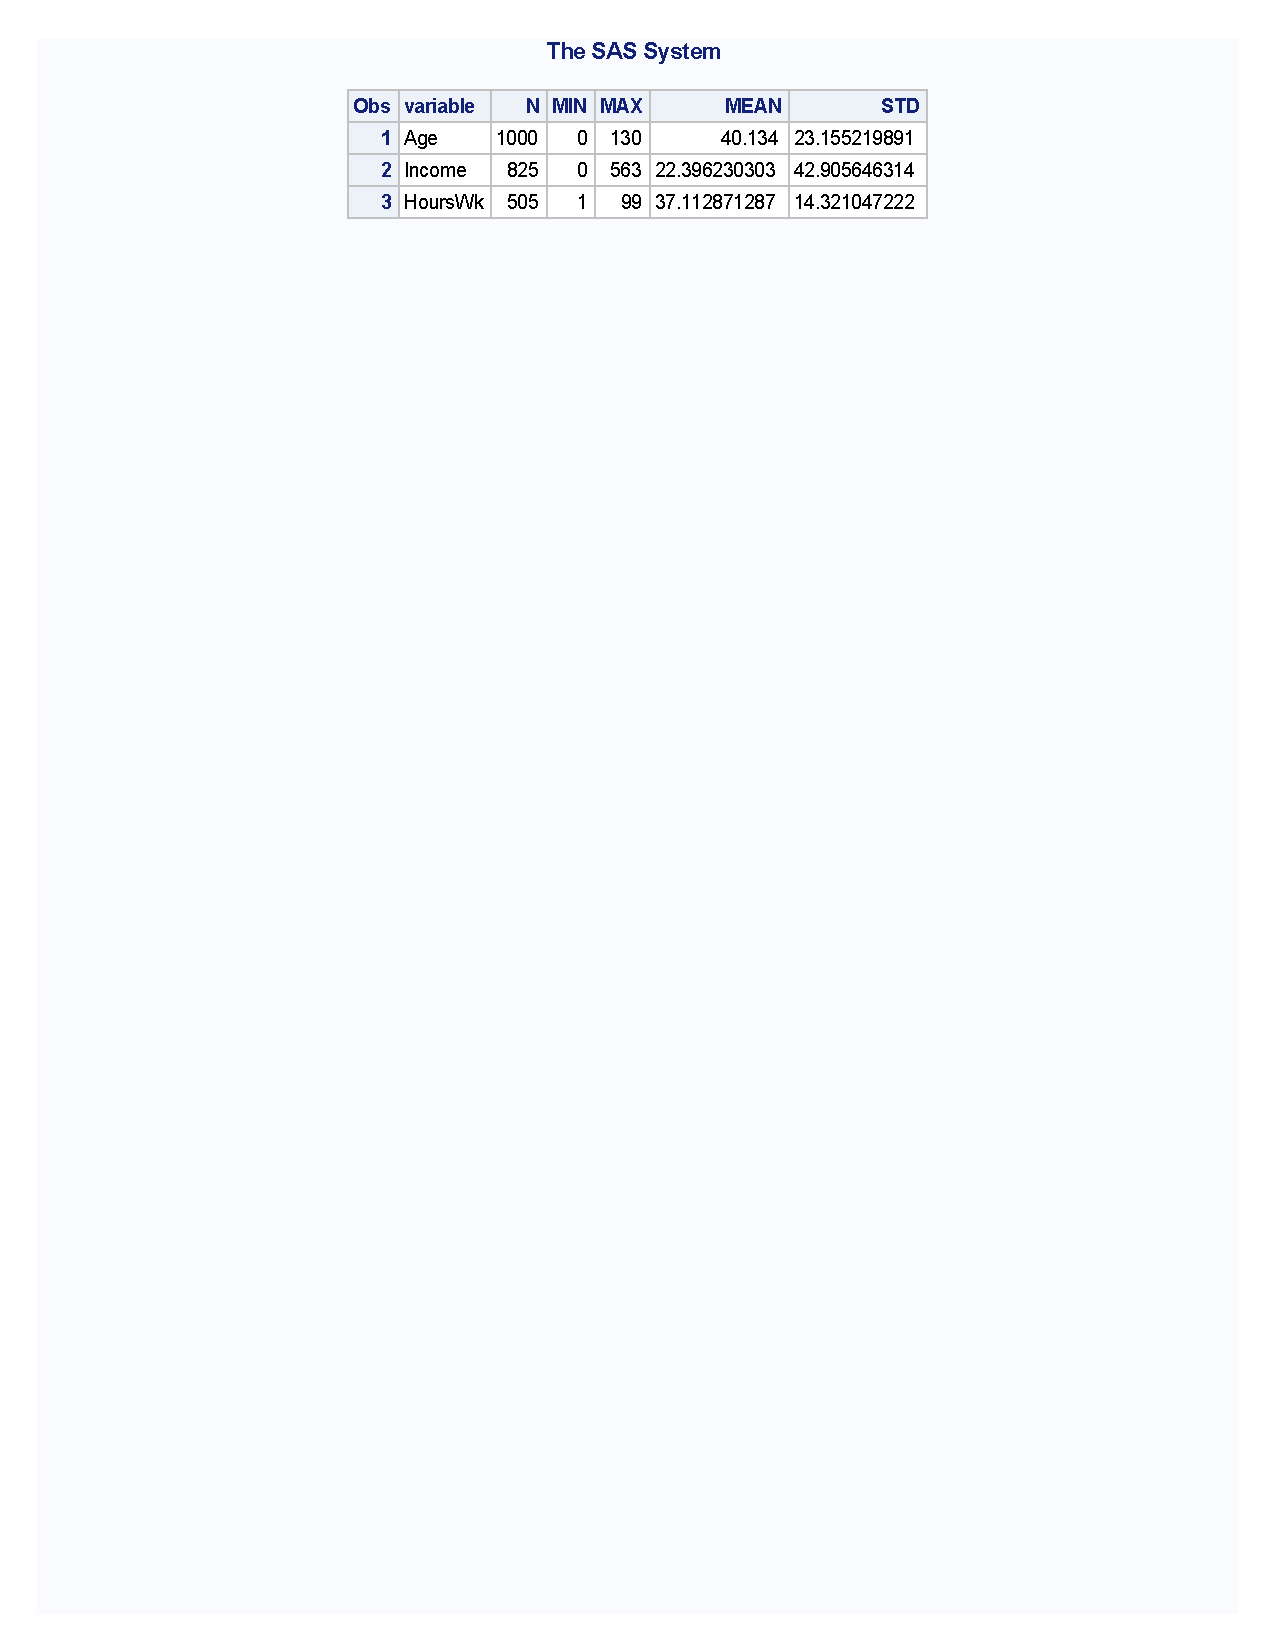
\includegraphics[trim=5cm 21cm 5cm 1.5cm,clip,width=1.0\textwidth]{L12_meanstransposed.pdf}
\emp
\end{frame}


\begin{frame}[fragile]
\ft{Discussion}
\bmp{0.5\textwidth}
\begin{craw}{.0}{Data we have}
Student  ID   Test1  Test2
Andrew  6545   94     91
Beth    1252   51     65
Charlie 1167   95     97
\end{craw}
\emp
\bmp{0.05\textwidth} \hspace{0.05in} \emp
\bmp{0.5\textwidth}
\begin{craw}{.0}{Data we want}
exams  Andrew  Beth  Charlie
Test1    94     51      95
Test2    91     65      97
\end{craw}
\emp
\vskip10pt
\bmp{0.5\textwidth}
\begin{code}{.0}
PROC TRANSPOSE
   DATA = datawehave
   OUT = datawewant
   NAME = \textcolor{OrangeRed}{\fbox{\ttt{1}}};
   ID     \textcolor{OrangeRed}{\fbox{\ttt{2}}};
   VAR    \textcolor{OrangeRed}{\fbox{\ttt{3}}};
run;
\end{code}
\emp
\bmp{0.05\textwidth} \hspace{0.05in} \emp
\bmp{0.5\textwidth}
\begin{clicker}{Fill in the SAS statements.}
\begin{enumerate}
\item %exams
\item %student
\item %test1 test2
\end{enumerate}
\end{clicker}
\emp
\end{frame}

\begin{frame}
\ft{Reshaping data}
\bi
\item Re-shaping data is commonly needed for longitudinal studies
\item Long format is required for longitudinal data analysis
\bi
\item[] Reshape data wide to long:
\item[] \url{https://stats.idre.ucla.edu/sas/modules/reshaping-data-wide-to-long-using-a-data-step/}
\ei
\item Wide format might be more useful for creating graphics or for paired analysis
\bi
\item[] Reshape data long to wide:
\item[] \url{https://stats.idre.ucla.edu/sas/modules/how-to-reshape-data-long-to-wide-using-proc-transpose/}
\ei
\ei
\end{frame}



%===========================================================================================================================
\section[PROC EXPORT]{PROC EXPORT}
%===========================================================================================================================
\subsection{}
\begin{frame}
\tableofcontents[currentsection, hideallsubsections]
\end{frame}

\begin{frame}[fragile]
\ft{PROC EXPORT}
\bmp{1.0\textwidth}
\footnotesize
\begin{code}{.0}
PROC EXPORT
   DATA = \emph{DataSetName}
   OUTFILE = "\emph{Computer Location/mydata.ext}"
   DBMS = \emph{identifier}
   REPLACE ;
RUN;
\end{code}
\emp
\vskip10pt
\bmp{0.10\textwidth} \hspace{0.05in} \emp
\bmp{0.90\textwidth}
\bi
\item[\fbox{\ttt{DATA=}}] specifies the SAS data set name you want to export
\item[\fbox{\ttt{OUTFILE=}}] takes computer location, data file name, and extension of the data file
\item[\fbox{\ttt{DBMS=}}] specifies type of data (e.g., \ttt{CSV}, \ttt{TAB}, \ttt{DLM})
\item[\fbox{\ttt{REPLACE}}] option overwrites an existing file called \emph{mydata.ext}
\ei
\emp
\end{frame}

\begin{frame}[fragile]
\ft{Example Code}
\bmp{0.65\textwidth}
\footnotesize
\begin{code}{.0}
DATA statstransposed2 ;
   SET statstransposed ;
   FORMAT mean 4.1 std 4.1 ;
RUN ;

PROC EXPORT
   DATA = statstransposed2
   OUTFILE = "&path.summarystats.csv"
   DBMS = CSV
   REPLACE ;
RUN;
\end{code}
\emp
\bmp{0.03\textwidth} \hspace{0.05in} \emp
\bmp{0.38\textwidth}
\bi
\item any format assigned to variables in the DATA step will be applied in the exported file for \ttt{.csv} or \ttt{.txt} files
\item exporting to \ttt{.xls} or \ttt{.xlsx} does not apply formats
\ei
\emp
\end{frame}

\end{document} 